\documentclass[10pt]{jarticle}
\usepackage{float}
\usepackage{adrobo_abst}
\usepackage[dvipdfmx]{graphicx}
\usepackage{amssymb,amsmath}
\usepackage{bm}
\usepackage[superscript]{cite}
\usepackage{enumerate}
\usepackage{url}
%\usepackage[absolute]{textpos}

\renewcommand\citeform[1]{(#1)}

\begin{document}
    
    \makeatletter
    \doctype{2021年度卒業論文概要}
  \title{      視覚と行動のEnd-to-End学習により経路追従行動を      オンラインで模倣する手法の提案}
        {(目標方向による経路選択の追加)}
    \etitle{A proposal for an online imitation method of path-tracking behavior   
    by end-to-end learning of vision and action}{(Add path selection by target direction.)}
    
    \author{18C1096\hspace{.5zw}春山健太}
    \eauthor{Kenta HARUYMA}
    
    \makeatother
    
    \abstract{We proposed a method for acquiring autonomous driving by End-to-End learning using camera images and target directions, which can select a specific path depending on the target direction.
    The effectiveness of the proposed method was verified by experiments using a simulator.
    }
    % カメラ画像と目標方向を用いたEnd-to-End学習を用いた走行において,目標方向によって特定の経路を選択する手法を提案した.実験により提案手法の有効性を検証した.
    \keywords{End-to-End Learning, Target Direction}
    
    \maketitle
    
    \supervisor{指導教員:林原靖男 教授}
    
    \section{緒\hspace{2zw}言}%===========================
    近年,カメラ画像に基づいた自律移動の研究が行われている.%\cite{nvidia}.
    Bojaskiら\cite{nvidia}は,人間のハンドル操作によるステアリング
    角度の模倣学習を行い,画像を用いて走行する手法を提案している.
    また岡田ら\cite{okada}は,
    LiDARとオドメトリのデータを入力とする
    ルールべースの制御器による経路追従行動を,
    カメラ画像によるEnd-to-End学習によって
    模倣する手法を提案している.
    % その制御器の出力する角速度とロボットに取り付けたカメラから取得したカメラ画像を用いて
    % 学習器の訓練を行い,学習後はカメラ画像のみを用いて自律移動を行う.
    % ルールベースの制御器を用いることでデータセットを自動的に収集し,
    % その経路追従行動を模倣する手法を提案している.
    上記の研究により,カメラ画像によるEnd-to-End学習を用いた走行において,
    ロボットが一定の経路を周回することが可能であると示されている.
    次に,\reffig{bunki}のような分岐路において,
    赤で示す「直進」と緑で示す「左折」などの特定の経路を
    選択する手法への拡張を検討する.
    カメラ画像のみでは,「どちらへ進むか」のような経路選択に必要な情報が不足している可能性がある.
    そこで,データセットへカメラ画像以外に,「直進」「左折」などの
    目標とする進行方向の情報(本研究では”目標方向”とする )を追加する
    ことで,特定の経路を選択可能であると考えられる.

    本稿では
    目標方向によって特定の経路を選択可能な,
    カメラ画像と目標方向を入力したEnd-to-End学習による自律走行を,
    獲得する手法を提案する.
    また提案手法に基づいて構築したシステムを用いた実験を行い,
    提案手法の有効性を検証する.
    \begin{center}
        \begin{figure}[h]
            \centering
            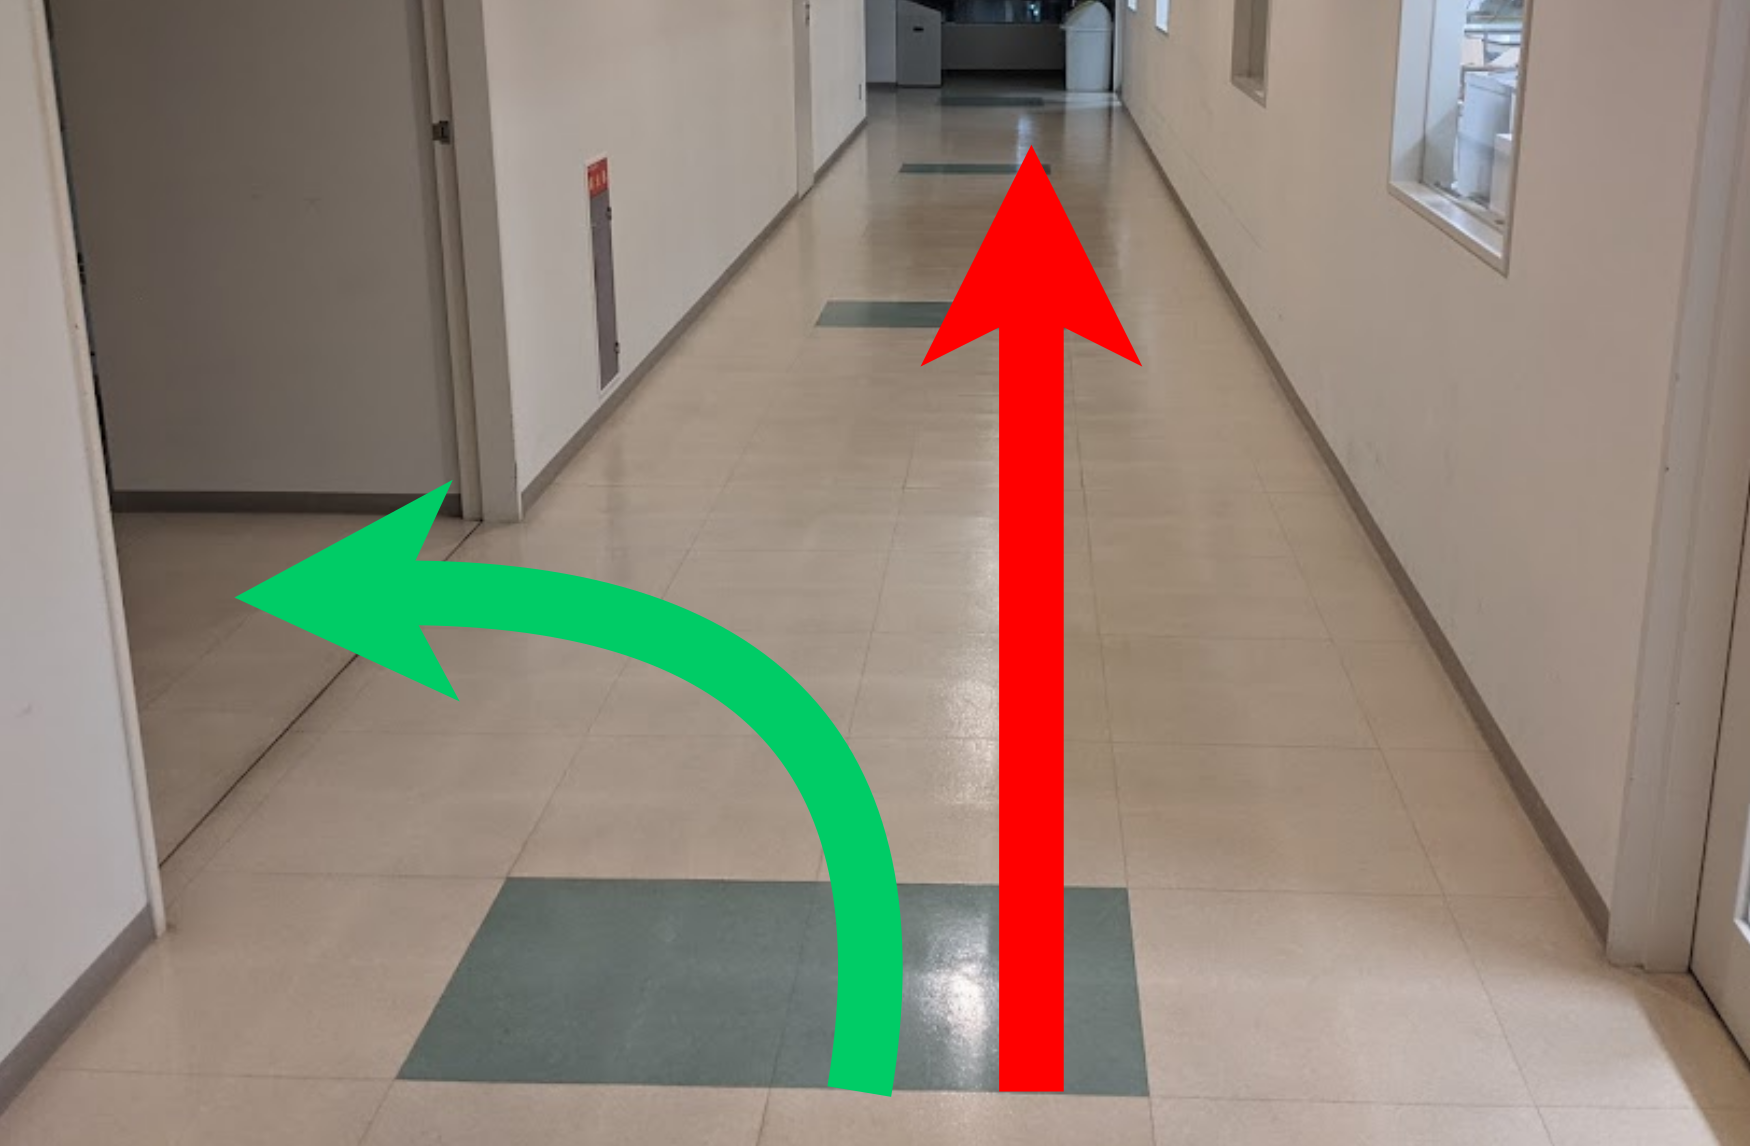
\includegraphics[width=5cm]{./fig/zyuzibunki.png}
            \caption{Cross road}
            \label{fig:bunki}
        \end{figure}
    \end{center}
    \section{提案手法}%===========================
    提案手法は学習器の訓練を行う「学習フェーズ」と
    訓練した学習器の出力を用いて走行する「テストフェーズ」の2つに分けられる.
    %=======================
    % \subsection{学習フェーズ}
    
    学習フェーズで用いるシステムを\reffig{system_learning}に示す.
    地図ベースの制御器は,
    ROS Navigation\_stack\cite{navigation}へ
    目標方向の生成機能を追加した,LiDARとオドメトリを入力とするルールベースの制御器である.
    目標方向は分岐路以外での「道なり」を示す(continue),
    分岐路を「直進(go straight)」,「左折(turn left)」,
    「右折(turn right)」の4つとする.
    これら4つの目標方向は,要素数4のOne-hotベクトルを用いて表現する.
    学習器の訓練は,次の流れを1stepとして設定したstep数の学習を行う.
    % 1)LiDARとオドメトリから得たデータを入力とする地図ベースの制御器の出力を用いて自律走行する.
    % 2)地図ベースの制御器の出力からヨー方向の角速度と目標方向,ロボットに取り付けた3つのカメラから
    % RGB画像を取得し,訓練データへ加える.
    % 3)訓練データ(入力:カメラ画像,目標方向 目標出力:角速度)を用いてEnd-to-End学習を行い,学習器の出力を記録.
    \begin{enumerate}
        \setlength{\parskip}{0cm} % 段落間
        \setlength{\itemsep}{0cm} % 項目間
        \item LiDARとオドメトリから得たデータを入力とする地図ベースの制御器の出力を用いて自律走行する
        \item 地図ベースの制御器の出力からヨー方向の角速度と目標方向,ロボットに取り付けた3つのカメラから
        RGB画像を取得し,訓練データへ加える.
        \item 訓練データ(入力:カメラ画像,目標方向 目標出力:角速度)を用いてEnd-to-End学習を行い,学習器の出力を記録
        \end{enumerate}
    \begin{center}
        \begin{figure}[h]
            \centering
            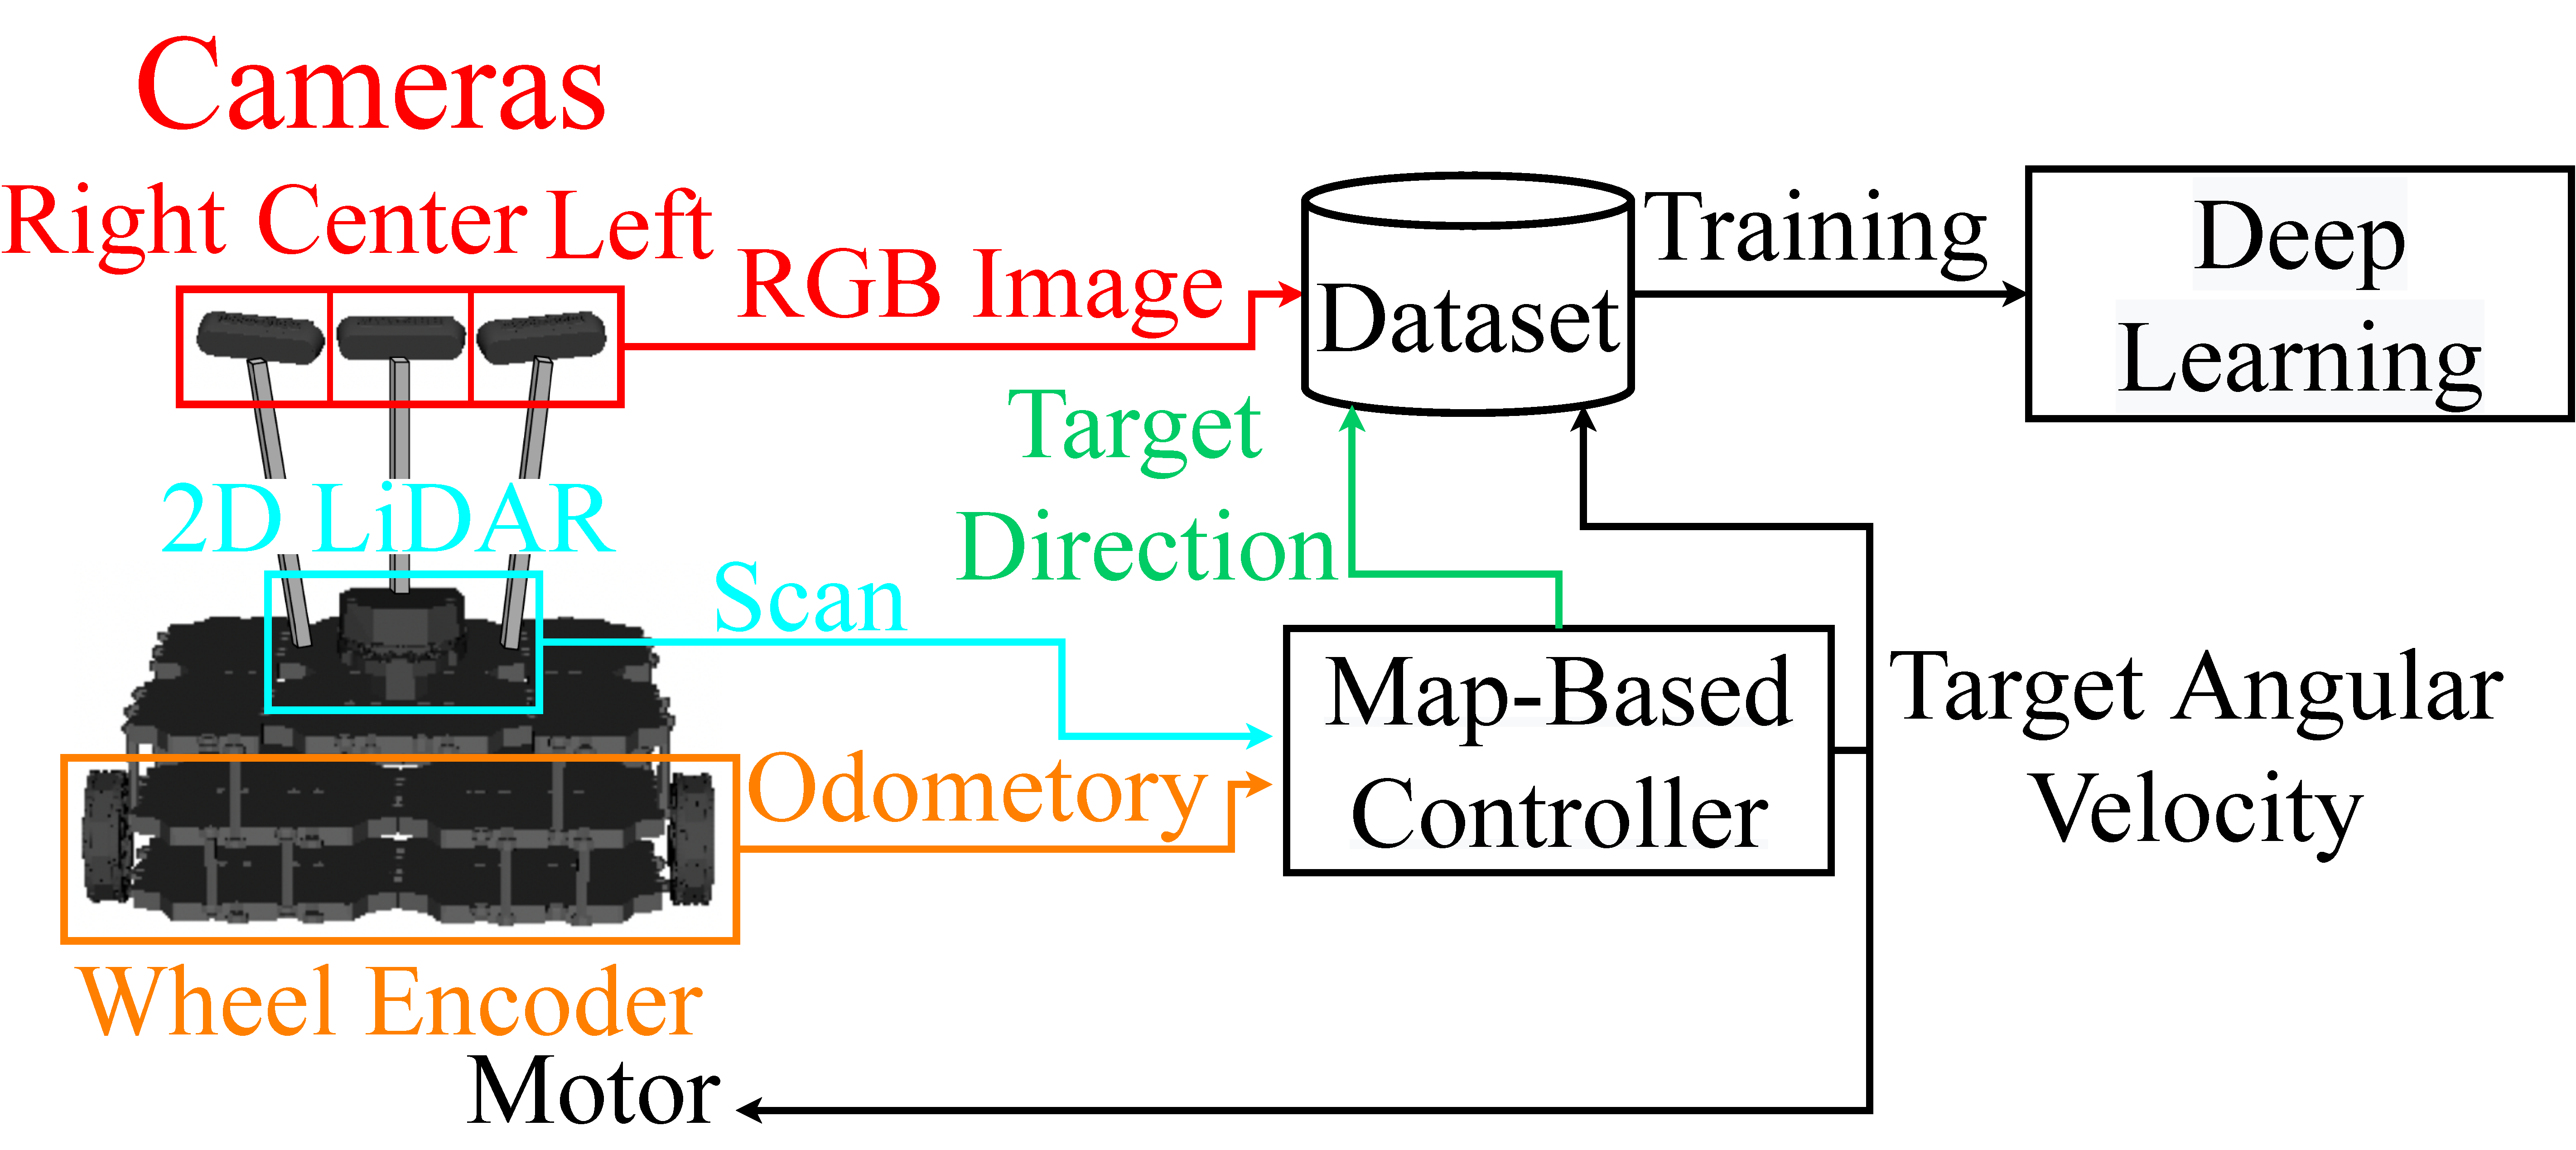
\includegraphics[width=0.46\textwidth]{./fig/system_learning.pdf}
            \caption{Learning phase}
            \label{fig:system_learning}
        \end{figure}
    \end{center}
    %=========================
    % \subsection{テストフェーズ}
    
    設定したstep数に達した場合,
    \reffig{system_test}に示すテストフェーズへ移行する.
    テストフェーズでの目標方向は,Joystickコントローラのボタンを用いて入力する.
    また並進速度は固定の値を用いる.
    テストフェーズにおける手順を下記に示す.
    
    \begin{enumerate}
    \setlength{\parskip}{0cm} % 段落間
    \setlength{\itemsep}{0cm} % 項目間
    \item ロボット中央のカメラからRGB画像 ,Joystickコントローラより目標方向のデータを取得.
    \item 取得したデータ (カメラ画像,目標方向)を学習器へ入力.
    \item 固定した並進速度,学習器の出力(角速度)を用いて走行.
    \end{enumerate}
    \begin{center}
        \begin{figure}[h]
            \centering
            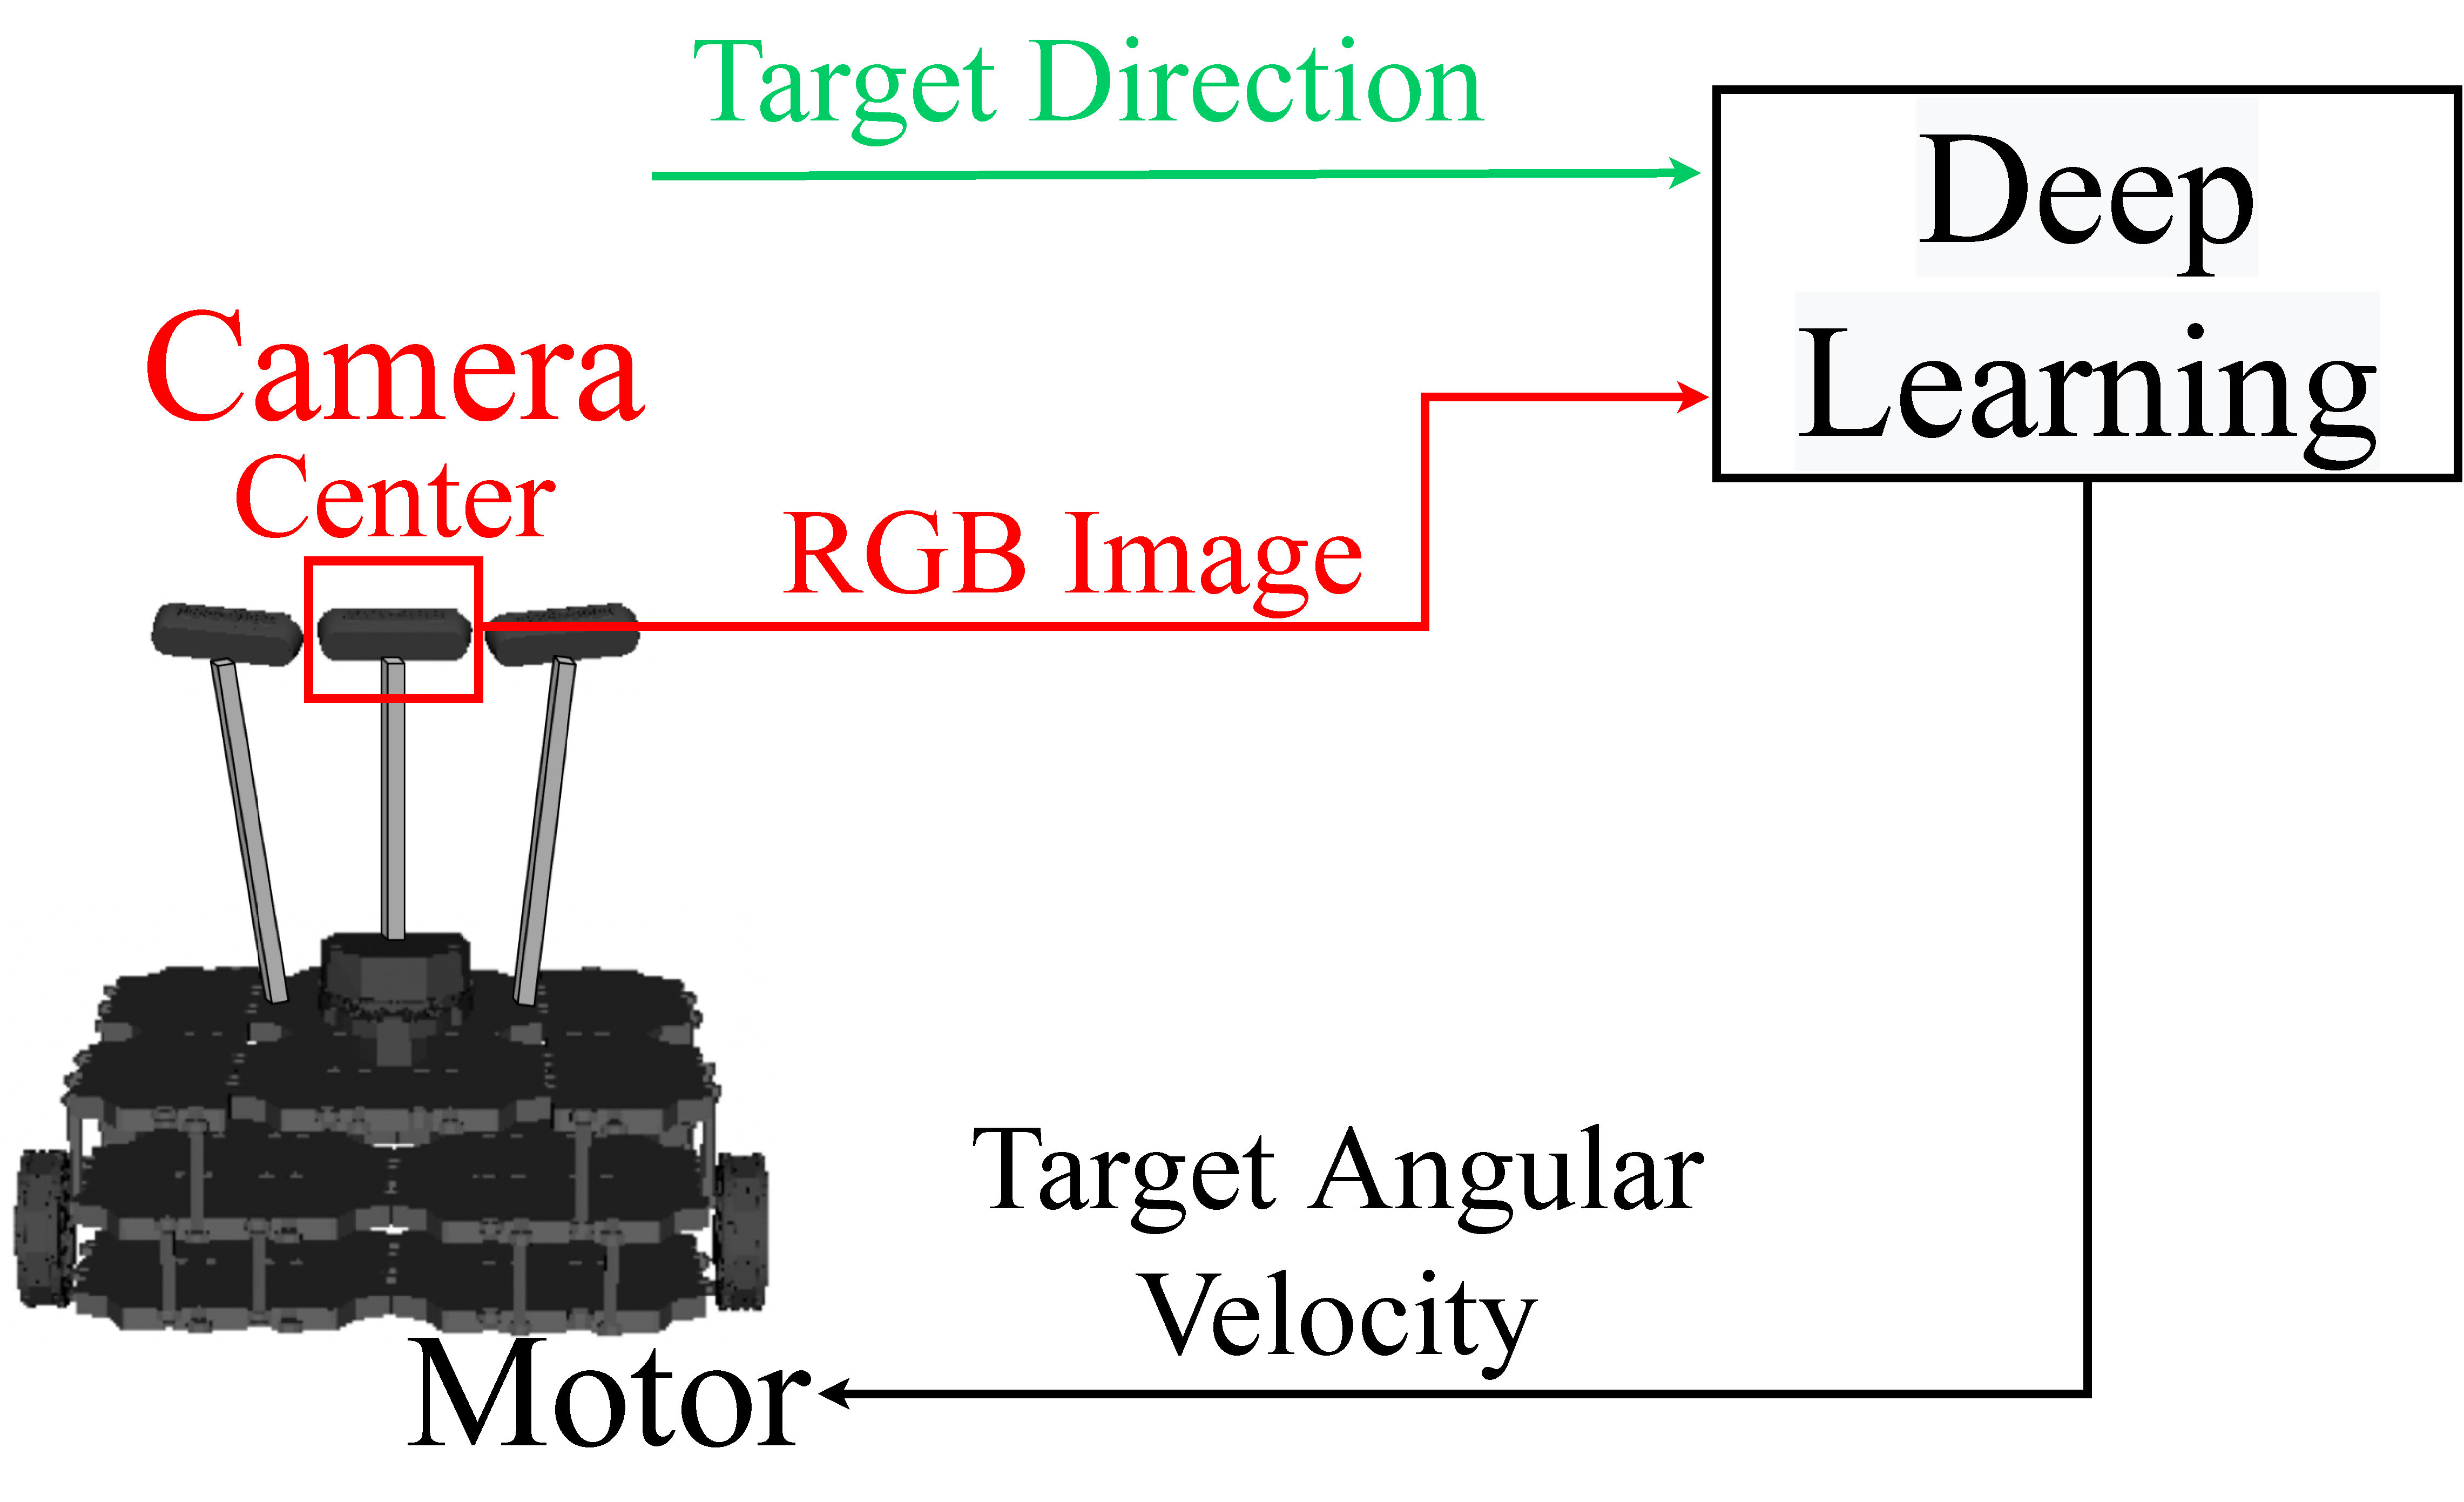
\includegraphics[width=5.7cm]{./fig/system_test.pdf}
            \caption{Test phase}
            \label{fig:system_test}
        \end{figure}
    \end{center}
    \vspace{-1zh}
    \section{実\hspace{2zw}験}%=========================検証
    提案手法の有効性の検証を検証するために
    3DロボットシミュレータGazebo上で実験を行う.
    環境は\reffig{exp}に示す道幅が2.5[m]の十字路を用いる.
    また,実験装置として\reffig{system_learning},\reffig{system_test}で示した
    Turtlebot3 waffleへカメラを3つ追加したモデルを用いる.
    実験は下記の手順でnを1,2,3と順に変更しながら,
    学習フェーズではstep数:4000[step],
    訓練フェーズでは並進速度は0.2[m/s]として各経路を5回
    繰り返し行う.
    \begin{enumerate}
        \setlength{\parskip}{0cm} % 段落間
        \setlength{\itemsep}{0cm} % 項目間
        \item 初期位置(緑)へロボットを設置.
        \item 緑-青-赤(n)の順で走行.
        \end{enumerate}
    目標方向は学習フェーズ,テストフェーズともに
    緑-青間(continue)
    青-赤(1)間(go straight)
    青-赤(2)間(turn left)
    青-赤(3)間(turn right)を入力する.
    実験条件はテストフェーズにおいて「壁に衝突せず,目標方向に対応した経路を選択」を成功,
    「目標方向とは異なったコースを選択する,または壁に衝突」を失敗とする.
    \begin{center}
        \begin{figure}[h]
            \centering
            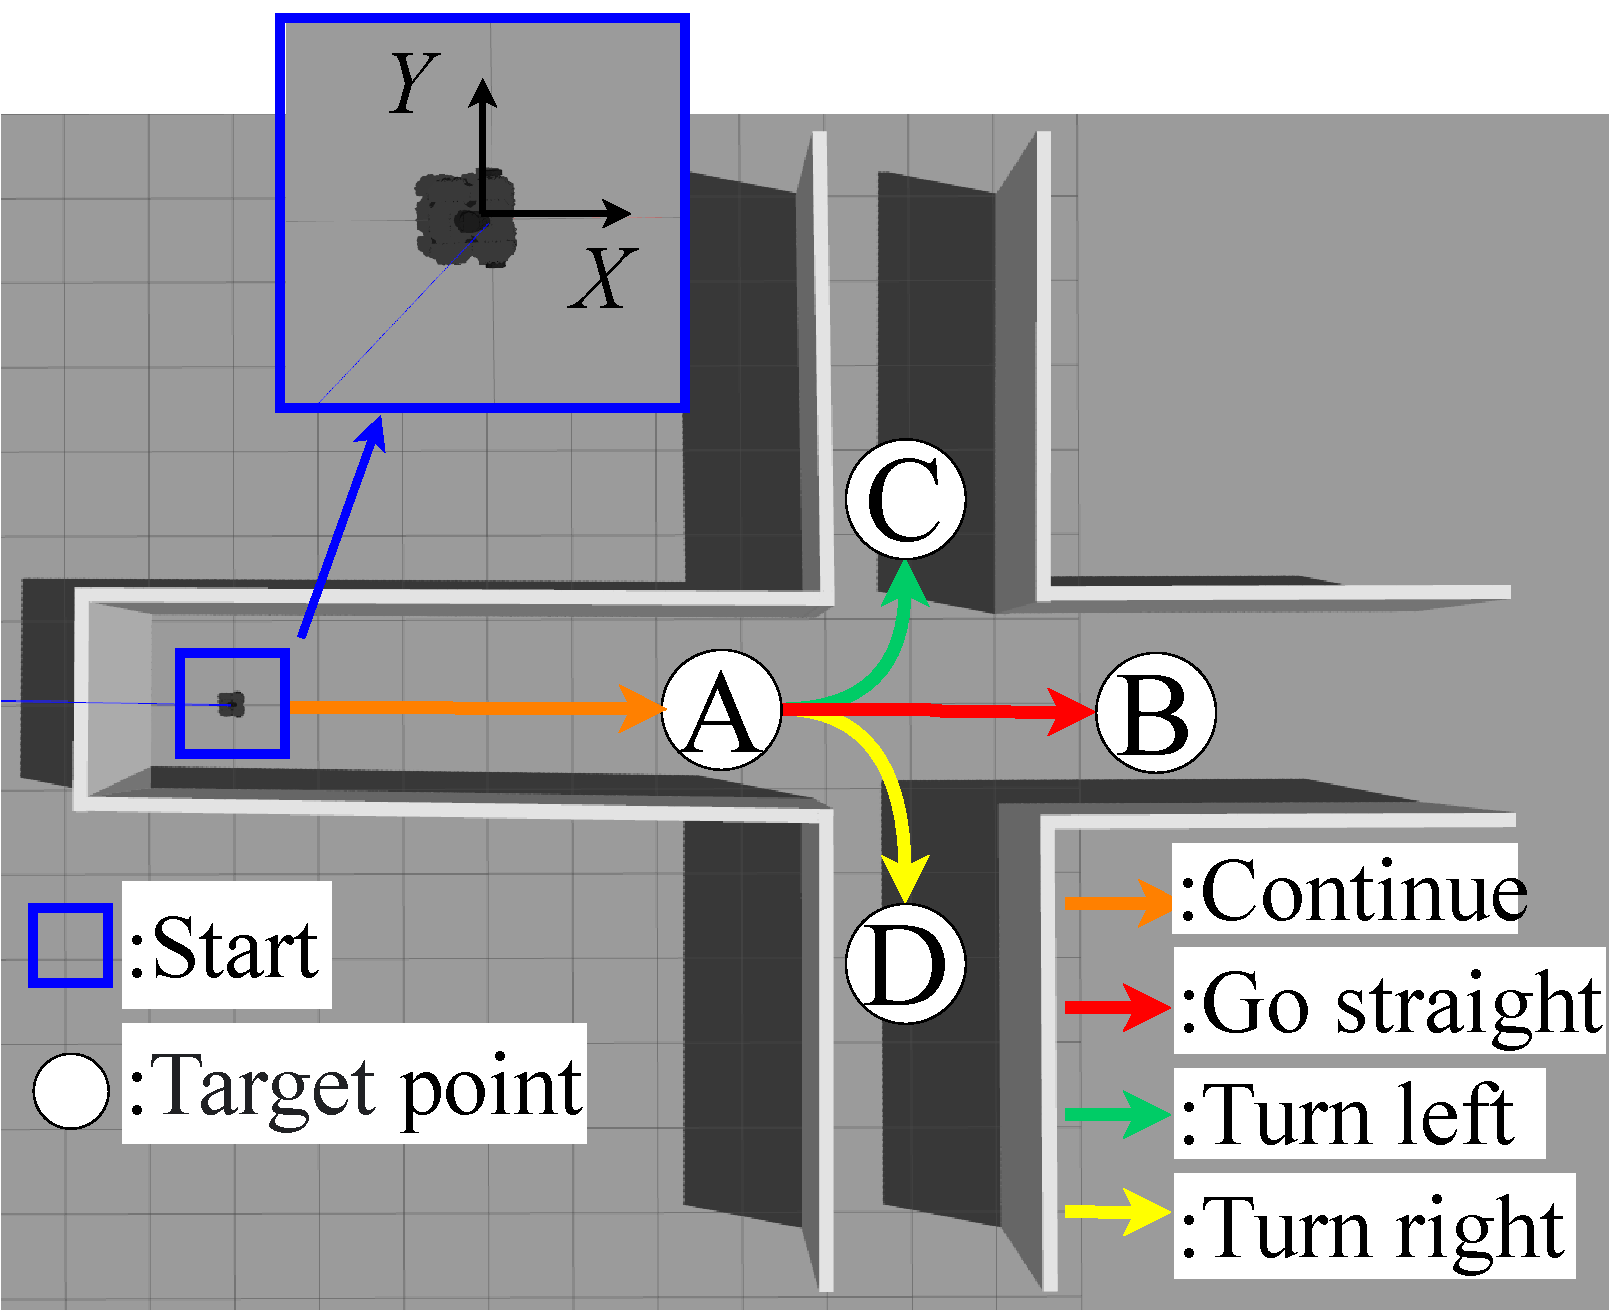
\includegraphics[width = 6cm]{./fig/zyuziroute.pdf}
            
            \caption{Environment for experiment}
            \vskip 0.1zh
            \label{fig:exp}
        \end{figure}
    \end{center}
    % \begin{enumerate}
    %     \setlength{\parskip}{0cm} % 段落間
    %     \setlength{\itemsep}{0cm} % 項目間
    %     \item 学習フェーズによって,学習器の訓練 ( 経路の学習 ) 行う
    %     ( 制御:地図べースの制御器の出力 )
    %     \item 設定した step 数を学習後,訓練フェーズへ移行
    %     ( 制御:学習器の出力 )
    %     \item コース内に設定した地点において目標方向のコマンドを入力,挙動を確認
    % \end{enumerate}
   \section{実験結果}
   実験結果を\reftab{suc}に示す.
   turn left(1)以外の各地点で全ての回数で特定の経路の選択に成功し,
   目標方向に対応した特定の経路を選択する行動が見られた.

    \section{結\hspace{2zw}言}%===========================
    本稿では,目標方向によって特定の経路を選択可能な,
    カメラ画像と目標方向を入力したEnd-to-End学習による自律走行を,
    獲得する手法を提案した.
    シミュレータを用いた実験により,提案手法の有効性を検証した.
    
    {\footnotesize
        \begin{thebibliography}{99}
            
            % \bibitem{工大2005}
            % 工大太郎: ``ロボットのしくみ'', 
            % 日本機械学会論文誌A, 
            % Vol.~108, No.~1034 (2005), pp.~1--2.
            
            \bibitem{nvidia}
            Mariusz Bojarski et al:``End to End Learning for Self-Driving Cars'',
            arXiv: 1604.07316,(2016)
            \bibitem{okada}
            岡田眞也, 清岡優祐, 上田隆一, 林原靖男:``視覚と行動の end-to-end 
            学習により経路追従行動をオンラインで模倣する手法の提案''
            SICE-SI2020予稿集,1147--1152,制御学会SI部門講演会(2020)
            \bibitem{navigation}
            ros-planning,navigation:
            \url{https://github.com/ros-planning/navigation}, 
            (参照日 2020年12月30日). 
            % \bibitem{Shibutani2004}
            % Y. Shibutani: ``Heinrich's Law Resulted Pattern Dynamics --Part2--'',
            % Proceedings of the 79th Kansai Branch Regular Meeting of the Japan Society of Mechanical Engineers,  
            % No.~04--05 (2004), pp.~205--206.
            
            % \bibitem{Handbook1979}
            % The Japan Society of Mechanical Engineers ed.: ``JSME Date Handbook: Heat Transfer'', 
            % (1979), p.~123, The Japan Society of Mechanical Engineers.
            
            % \bibitem{Kikuchi2017}
            % K. Kikuchi, M. Miura, K. Shibata, J. Yamamura: ``Soft Landing Condition for Stair-climbing Robot with Hopping Mechanism'', 
            % Journal of JSDE, Vol.~53, No.~8 (2018), pp.~605--614, \url{https://doi.org/10.14953/jjsde.2017.2774}.
        \end{thebibliography}
    }
    \begin{table}[H]
        \caption{Number of successes experiment  point}
        \label{tab:suc}
        \begin{center}
            \vskip -1zh
            \begin{tabular}{|c|c|}
                \hline
                Target direction and Point & Number of successes\\ \hline
                continue  & $5/5$ \\ \hline
                go straihgt (1) & $5/5$ \\ \hline
                turn left (2) & $4/5$ \\ \hline
                turn right (3) & $5/5$ \\ \hline
            \end{tabular}
        \end{center}
    \end{table}
        
   
    \vspace{5truemm}
    
    \normalsize
    
\end{document}
